\documentclass[aspectratio=169,11pt]{beamer}
\usepackage{teaching_slides}

\title[L13c - Count Data]{ Econometrics I}
\subtitle{Lecture 13c: Count Data}
\author{Chris Conlon \\NYU Stern}
\date{Fall 2026}

% Expanded Fall 2026 from the older Count Data deck: adds exposure/offsets, zero inflation,
% AIC/BIC/Vuong model comparison (folded in from the retired L12a deck), and Poisson
% pseudo-ML with fixed effects. The text-as-data section was removed.
% Readings: Wooldridge Ch. 19; Cameron & Trivedi Ch. 20.
% Figures/tables simulated with known ground truth: ldv_sims.R (Part C).

\begin{document}
\maketitle

\begin{frame}{Count data}
\begin{itemize}
	\item Dependent variable is a count: $y \in \{0, 1, 2, \dots\}$.
	\medskip
	\item Examples: purchases per customer per quarter, store visits, insurance claims, patents per firm,
	doctor visits, customer complaints, app sessions, number of children.
	\medskip
	\item Three things a linear model gets wrong: predictions go negative, the variance grows with the mean
	(heteroskedasticity by construction), and the pile of zeros is not a normal residual.
	\medskip
	\item Plan: Poisson as the baseline and why it is robust; overdispersion and the negative binomial;
	exposure; zero inflation and how to choose among models; counts in panels with fixed effects.
	\medskip
	\item Readings: Wooldridge Ch.~19; Cameron and Trivedi Ch.~20.
\end{itemize}
\end{frame}


\begin{frame}{Poisson distribution}
\begin{itemize}
	\item \alert{Poisson process}: events happen independently over time at rate $\lambda$
	per unit time. The \alert{Poisson distribution} gives the distribution of the number of events.
	\smallskip
	\item Probability mass:\[
		\Pr\left(Y=y \mid \lambda\right) = \frac{e^{-\lambda}\lambda^{y}}{y!}
	\]
	One parameter:\begin{align*}
	\E\left[y\right] & = \lambda \\
	\Var\left[y\right] &= \lambda
	\end{align*}
	\item \alert{Equidispersion}, mean $=$ variance, is a strong restriction. Real count data are almost
	always \alert{overdispersed} (variance $>$ mean), which is the negative binomial's cue.
\end{itemize}
\end{frame}


\begin{frame}{Poisson distribution}
\begin{center}
 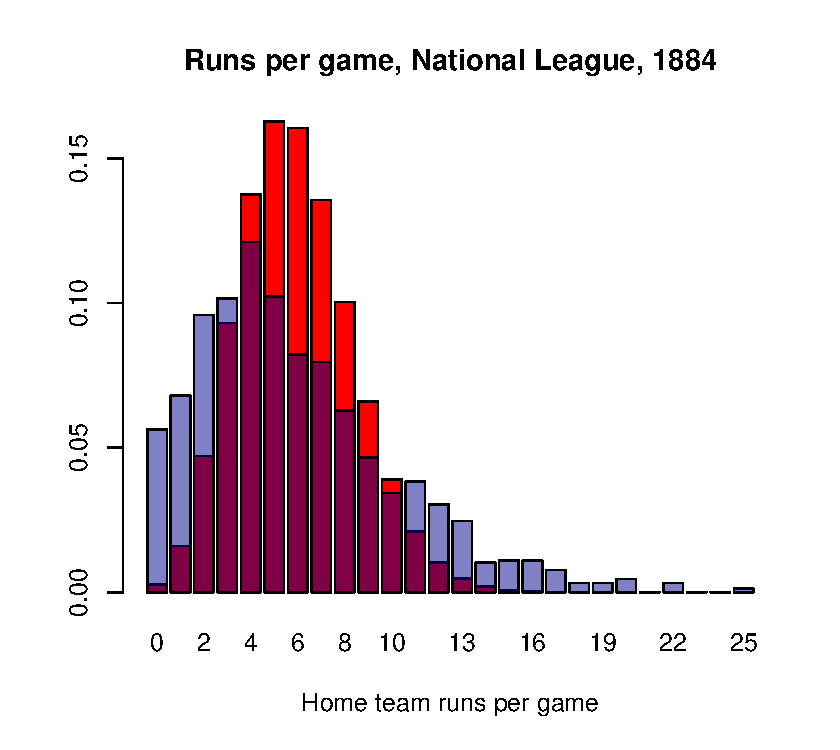
\includegraphics[height=.7\textheight]{./resources/home_team_runs}
\end{center}
{\small
Plotted Poisson distribution (red) is for $\lambda$ equal to the average runs per game. \\
Empirical probability mass function is in blue.
}
\end{frame}


\begin{frame}{Poisson regression (MLE)}
\begin{itemize}
\item  Let the rate vary with observables:\[
	\lambda \left(x\right) = \E\left[y \mid x\right] = \exp\left(x'\beta\right),
	\]
	which keeps $\lambda(x) > 0$ and makes $\beta_j$ a semi-elasticity.
	\medskip
	\item Log likelihood from the Poisson pmf:\begin{align*}
	\ell\left(\beta\right) &=  \sum_{i=1}^{n}\left\{-\exp\left(x_{i}'\beta \right)+ y_i x_{i}' \beta - \ln y_{i}!\right\}
	\end{align*}
	\item First-order condition:\begin{align*}
	  \sum_{i=1}^{n}\left(y_i -\exp\left(x_{i}'\beta \right) \right) x_{i} = 0 .
	\end{align*}
	\item Globally concave: Newton's method converges from anywhere.
\end{itemize}
\end{frame}


\begin{frame}{Poisson: marginal effects}
\begin{itemize}
\item Marginal effects:\[
	\frac{\partial \E\left[y \mid x\right]}{\partial x_j} = \exp\left( x'\beta\right) \beta_j =
	\E\left[y \mid x\right] \beta_j
\]
	\item Equivalently,\[
	\frac{1}{\E\left[y \mid x\right] }\frac{\partial \E\left[y \mid x\right]}{\partial x_j}  = \beta_j,
\]
	so $\beta_j$ is the \alert{proportional change in the mean} for a unit change in $x_j$. For a dummy,
	$e^{\beta_j} - 1$ is the exact proportional change.
	\medskip
	\item Compare the transformations deck (Week 2): this is the ``log-linear'' interpretation
	\emph{without} taking logs of $y$, so zeros are not a problem. Hold that thought for the panel section.
\end{itemize}
\end{frame}


\begin{frame}{Poisson is robust: consistency needs only the mean}
\begin{itemize}
	\item The first-order condition
	$\sum_i \left(y_i -\exp\left(x_{i}'\beta \right) \right) x_{i} = 0$
	is a moment condition. It holds in the population whenever
	$\E\left[y_i \mid x_i\right] = \exp\left(x_{i}'\beta\right)$.
	\medskip
	\item So the Poisson MLE is consistent for $\beta$ \alert{even if the data are not Poisson}: overdispersed,
	underdispersed, zero-heavy, whatever. Only the conditional mean has to be right. (Gourieroux, Monfort and
	Trognon 1984: \alert{pseudo-maximum likelihood}.)
	\medskip
	\item What breaks is the \emph{variance}: the MLE standard errors assume $\Var[y \mid x] = \E[y \mid x]$.
	With overdispersion they are too small, often by a lot.
	\medskip
	\item Fix: sandwich (robust) standard errors, Week 3. In \texttt{fixest}, \texttt{fepois} with
	\texttt{vcov = "hetero"} or a cluster.
	\medskip
	\item This is why Poisson regression has become the default for any non-negative outcome with zeros,
	including dollar amounts (Santos Silva and Tenreyro 2006, in trade; now everywhere).
\end{itemize}
\end{frame}


\begin{frame}{Exposure}
\begin{itemize}
	\item Counts are usually \emph{per something}: purchases per \alert{months active}, claims per
	\alert{policy-year}, patents per \alert{R\&D dollar}, accidents per \alert{miles driven}.
	\medskip
	\item If events arrive at rate $\lambda(x)$ per unit of exposure $E_i$, then
	$\E[y_i \mid x_i, E_i] = E_i \exp(x_i'\beta) = \exp(x_i'\beta + \ln E_i)$.
	\medskip
	\item So include $\ln E_i$ as a regressor with its coefficient \alert{fixed at one}: an \alert{offset}.
	Everything else is unchanged; $\beta$ is now the effect on the \emph{rate}.
	\medskip
	\item Estimating the coefficient on $\ln E_i$ instead of fixing it is a test of proportionality;
	fine as a check, but the offset is the model.
	\medskip
	\item The running example below has customers active for one, two, or three months of the quarter.
\end{itemize}
\end{frame}


\begin{frame}{Overdispersion and the negative binomial}
\begin{itemize}
\item  Put unobserved heterogeneity in the rate:
\begin{align*}
	y \mid \lambda, \nu & \sim \text{Poisson}\left[\lambda \nu \right], \qquad
	\nu \sim \text{Gamma}\left[\text{mean } 1, \text{ variance } \alpha \right].
\end{align*}
	Integrating out $\nu$: $y$ is \alert{negative binomial} with mean $\lambda$ and variance $\lambda + \alpha\lambda^2$.
	\medskip
	\item Same mean as Poisson. Extra variance grows with $\lambda^2$: heavy buyers are \emph{much} more
	variable. $\alpha = 0$ is Poisson, so an LR test of $\alpha = 0$ is a test for overdispersion.
	\medskip
	\item The classic description (failures before $r$ successes) is the same distribution with
	$r = 1/\alpha$ and $p = \lambda\alpha/(1 + \lambda\alpha)$; useful for simulation.
	\medskip
	\item \alert{When to bother.} If you only want $\beta$ in the conditional mean, Poisson with robust
	standard errors already has it. Estimate the NB when you need the \emph{distribution}: predicting the
	share of customers with zero or ten-plus purchases, simulating, or pricing risk.
\end{itemize}
\end{frame}


\begin{frame}{Running example: purchases per customer-quarter}
\begin{itemize}
	\item $4{,}000$ customers. Covariates: \alert{promo} exposure (half) and standardized \alert{tenure};
	exposure is months active in the quarter ($1$, $2$, or $3$).
	\medskip
	\item Ground truth, in three layers:
	\begin{align*}
		\lambda_i &= E_i \exp(-0.5 + \alert{0.6}\cdot\text{promo}_i + \alert{0.2}\cdot\text{tenure}_i)\cdot \nu_i,
		\qquad \nu_i \sim \text{Gamma}(\text{var } \alert{0.8}) \\
		y_i &= 0 \text{ with probability } \alert{0.25} \text{ (never buys this category), else Poisson}(\lambda_i).
	\end{align*}
	\medskip
	\item Sample: mean $1.3$, variance $4.9$, and $55\%$ zeros. Overdispersed, zero-heavy: ordinary.
	\medskip
	\item Fit Poisson, negative binomial, and a zero-inflated negative binomial, and compare.
\end{itemize}
\end{frame}


\begin{frame}{Zero inflation and hurdles}
\begin{itemize}
	\item Two reasons for a zero: the customer \emph{could} have bought and did not (a Poisson zero), or
	is \emph{not in the market} (a structural zero). With both, no single rate fits zeros and positives.
	\item \alert{Zero-inflated} model: with probability $\pi_i$ the count is zero for sure; otherwise
	it is Poisson or NB. The likelihood is a mixture:
	\begin{align*}
		\Pr(y = 0) = \pi + (1 - \pi)\,f(0 \mid \lambda), \qquad \Pr(y = k) = (1 - \pi)\,f(k \mid \lambda),\ k \ge 1 .
	\end{align*}
	Let $\pi_i$ depend on covariates through a logit if ``who is in the market'' is itself the question.
	\item \alert{Hurdle} model: a binary model for $y > 0$, then a \emph{truncated} count model for
	$y \ge 1$; all zeros are structural and the two parts estimate separately.
	\item Neither is in \texttt{fixest}; the likelihood is ten lines in \texttt{optim} (workbook). Same idea
	as the Tobit deck's two-part model: if the zeros are a different decision, give them their own equation.
\end{itemize}
\end{frame}


\begin{frame}{Fit: observed versus predicted distributions}
\begin{center}
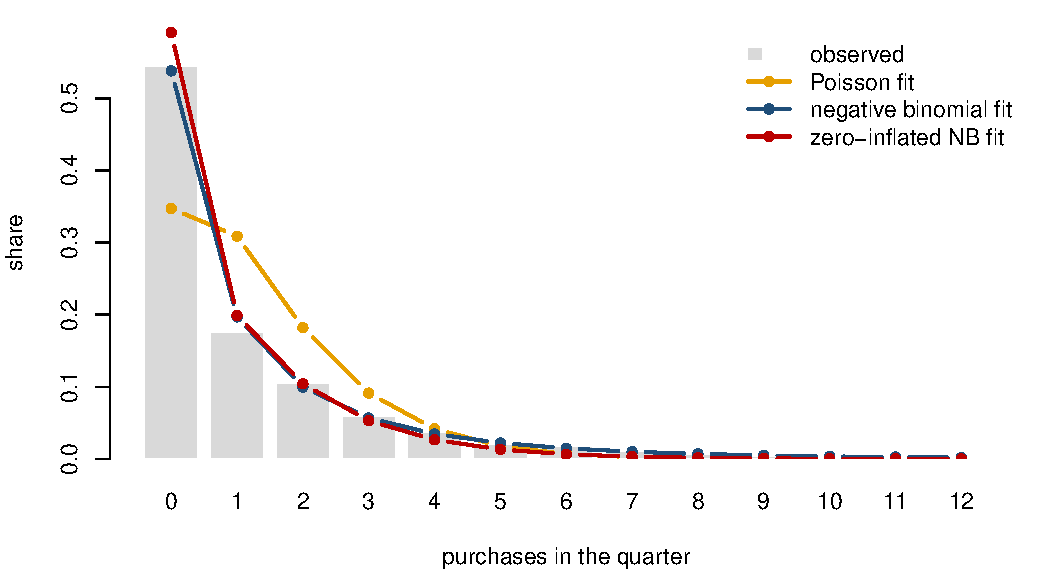
\includegraphics[width=.66\textwidth]{fig_count_fit.pdf}
\end{center}
\vspace{-.3cm}
{\small The Poisson fit has too few zeros and too few large counts, the signature of overdispersion. NB fixes the
tail; the zero-inflated NB fixes the zeros as well. All three have nearly the same $\hat\beta$, which is the
robustness point: the \emph{mean} was never the problem.}
\end{frame}


\begin{frame}{Choosing among models: AIC, BIC, and Vuong}
Three models with different likelihoods, not all nested. Tools:
\begin{itemize}
	\item \alert{Likelihood ratio} for nested pairs: Poisson within NB ($\alpha = 0$, on the boundary: halve the $p$-value).
	\item \alert{Information criteria} for any pair: $\text{AIC} = -2\ell + 2k$, $\text{BIC} = -2\ell + k\ln n$.
	AIC estimates expected out-of-sample fit (Kullback--Leibler distance to the truth); BIC penalizes harder
	and picks the true model with probability $\to 1$ if it is a candidate. Lower is better.
	\item \alert{Vuong (1989)} for non-nested pairs: with $m_i = \ln f_A(y_i) - \ln f_B(y_i)$,
	$z = \sqrt{n}\,\bar m / s_m \xrightarrow{d} N(0,1)$ under $H_0$ that the two models are equally
	close to the truth. A $t$-test on pointwise log-likelihood differences; positive favors $A$; neither
	model has to be true.
	\item None of these tests whether $\beta$ is right. They rank \emph{distributions}: use them for
	prediction and simulation, not to decide whether an effect exists.
\end{itemize}
\end{frame}


\begin{frame}{Estimates on the simulated customers}
\begin{center}
\scriptsize
\begin{tabular}{lcccc}\toprule
 & Poisson & Poisson, robust SE & Negative binomial & Zero-inflated NB \\ \midrule
Promo (truth $= 0.6$ among buyers) & 0.631 & 0.631 & 0.620 & 0.615 \\
 & (0.029) & (0.051) & (0.051) & (0.049) \\
Tenure (truth $= 0.2$) & 0.213 & 0.213 & 0.204 & 0.203 \\
 & (0.014) & (0.026) & (0.026) & (0.024) \\
Overdispersion $\alpha$ (truth $= 0.8$) & 0 (imposed) & --- & 1.64 & 0.85 \\
Never-buyer share $\pi$ (truth $= 0.25$) & --- & --- & --- & 0.24 \\
Log-likelihood & -7200.5 & (same) & -5827.1 & -5812.9 \\
AIC / BIC & 14407 / 14426 & & 11662 / 11687 & 11636 / 11667 \\
Vuong, ZINB vs.\ NB & & & \multicolumn{2}{c}{$z = 2.73$ (favors ZINB)}  \\
\bottomrule\end{tabular}

\end{center}
\begin{itemize}
	\item All four columns agree on the mean effects; the Poisson MLE standard errors are half the robust ones.
	\item NB alone blames the excess zeros on overdispersion ($\hat\alpha = 1.6$ vs.\ $0.8$); the
	zero-inflated version separates the two, and AIC, BIC, and Vuong all prefer it.
\end{itemize}
\end{frame}


\begin{frame}{Counts in panels: fixed effects work here}
\begin{itemize}
	\item Customers $\times$ quarters, with a customer effect $\eta_i$ in the rate:
	$\E[y_{it} \mid x_{it}, \eta_i] = \exp(x_{it}'\beta + \eta_i)$.
	\medskip
	\item Unlike the logit (incidental parameters, Week 12), the Poisson fixed-effects MLE is
	\alert{consistent for fixed $T$}: conditioning on $\sum_t y_{it}$ removes $\eta_i$ exactly, and the
	conditional MLE coincides with the plain MLE with customer dummies (Hausman, Hall and Griliches 1984;
	Lancaster 2000). Same robustness: only the mean has to be right.
	\medskip
	\item Practical facts: customers with $y_{it} = 0$ in every period drop out (they carry no information
	about $\beta$; \texttt{fepois} tells you how many). Cluster by customer.
	\medskip
	\item The alternative people reach for is OLS on $\ln(1 + y_{it})$ with customer FE. The transformations
	deck (Week 2) explained why $\ln(1+y)$ has no units-invariant interpretation; here is what it does to a
	known effect.
\end{itemize}
\end{frame}


\begin{frame}{Poisson pseudo-ML with fixed effects versus $\ln(1+y)$}
Simulated: $1{,}500$ customers $\times$ $8$ quarters. Heavy buyers ($\eta_i$ high) are targeted with more
promotions. True promo effect: $0.6$ log points on the rate.
\begin{center}
\small
\begin{tabular}{lcccc}\toprule
 & Poisson, no FE & Poisson + customer FE & OLS $\ln(1+y)$ + FE & OLS $\ln y$ ($y>0$) + FE \\ \midrule
Promo (truth $= 0.6$ log points) & -0.678 & 0.590 & 0.222 & 0.253 \\
 & (0.027) & (0.024) & (0.010) & (0.015) \\
Observations & 12000 & 11200 & 12000 & 5365 \\
Share of zeros in $y$ & \multicolumn{4}{c}{0.54}  \\
\bottomrule\end{tabular}

\end{center}
\medskip
\begin{itemize}
	\item Without FE the targeting flips the sign. With FE, Poisson recovers $0.6$.
	\item $\ln(1+y)$ with the same FE gets a third of the effect, and dropping the zeros does no better.
	Neither number is an elasticity of anything.
\end{itemize}
\end{frame}


\begin{frame}[fragile]{In practice}
Everything except zero inflation is \texttt{fixest}:
\begin{lstlisting}
fepois(y ~ promo + tenure, d, offset = ~log(months), vcov = "hetero")    # Poisson, robust SE
fenegbin(y ~ promo + tenure, d, offset = ~log(months))                    # negative binomial (+ theta)
fepois(y ~ promo | id, panel, vcov = ~id)                                 # Poisson with customer FE
\end{lstlisting}
Zero-inflated NB by hand (the workbook fills in the details):
\begin{lstlisting}
nll <- function(th) { la <- exp(X %*% th[1:3] + off); a <- exp(th[4]); pi <- plogis(th[5])
  f <- dnbinom(y, size = 1/a, mu = la)
  -sum(ifelse(y == 0, log(pi + (1 - pi) * f), log(1 - pi) + log(f))) }
optim(start, nll, method = "BFGS", hessian = TRUE)
\end{lstlisting}
\begin{itemize}
	\item Python: \texttt{pf.fepois} in \texttt{pyfixest}; \texttt{statsmodels} has NB, zero-inflated, and hurdle models.
\end{itemize}
\end{frame}


\begin{frame}{Recap}
\begin{itemize}
	\item Poisson regression is a model of the \emph{conditional mean} with a log link. It is consistent
	whenever the mean is right, Poisson or not. Use robust standard errors.
	\medskip
	\item Exposure goes in as an offset. Overdispersion goes in as gamma heterogeneity (negative binomial)
	when you need the distribution, not just the mean.
	\medskip
	\item Excess zeros: ask whether they are a different decision. Zero-inflated and hurdle models give them
	their own equation. AIC, BIC, and Vuong rank the distributions; they do not test $\beta$.
	\medskip
	\item In panels, Poisson with unit fixed effects is consistent at fixed $T$ and is the right replacement
	for $\ln(1+y)$ regressions.
\end{itemize}
\end{frame}


\begin{frame}{Workbook time}
\texttt{inclass\_session13.Rmd}:
\begin{enumerate}
	\item Tobit: reproduce the estimates table; then add heteroskedasticity to $\varepsilon$ and watch the
	probit check fail.
	\item Durations: reproduce Kaplan--Meier and Cox; then build the person-month data and confirm the
	cloglog with month dummies gives the same $\hat\beta$.
	\item Counts: reproduce the Poisson/NB/ZINB comparison and the panel table; then make promo exposure
	\emph{independent} of $\eta_i$ and see which columns change.
\end{enumerate}
\end{frame}

\end{document}
